\documentclass{subfiles}

\begin{document}
	\begin{figure*}[htp]
		\centering
		\subfloat{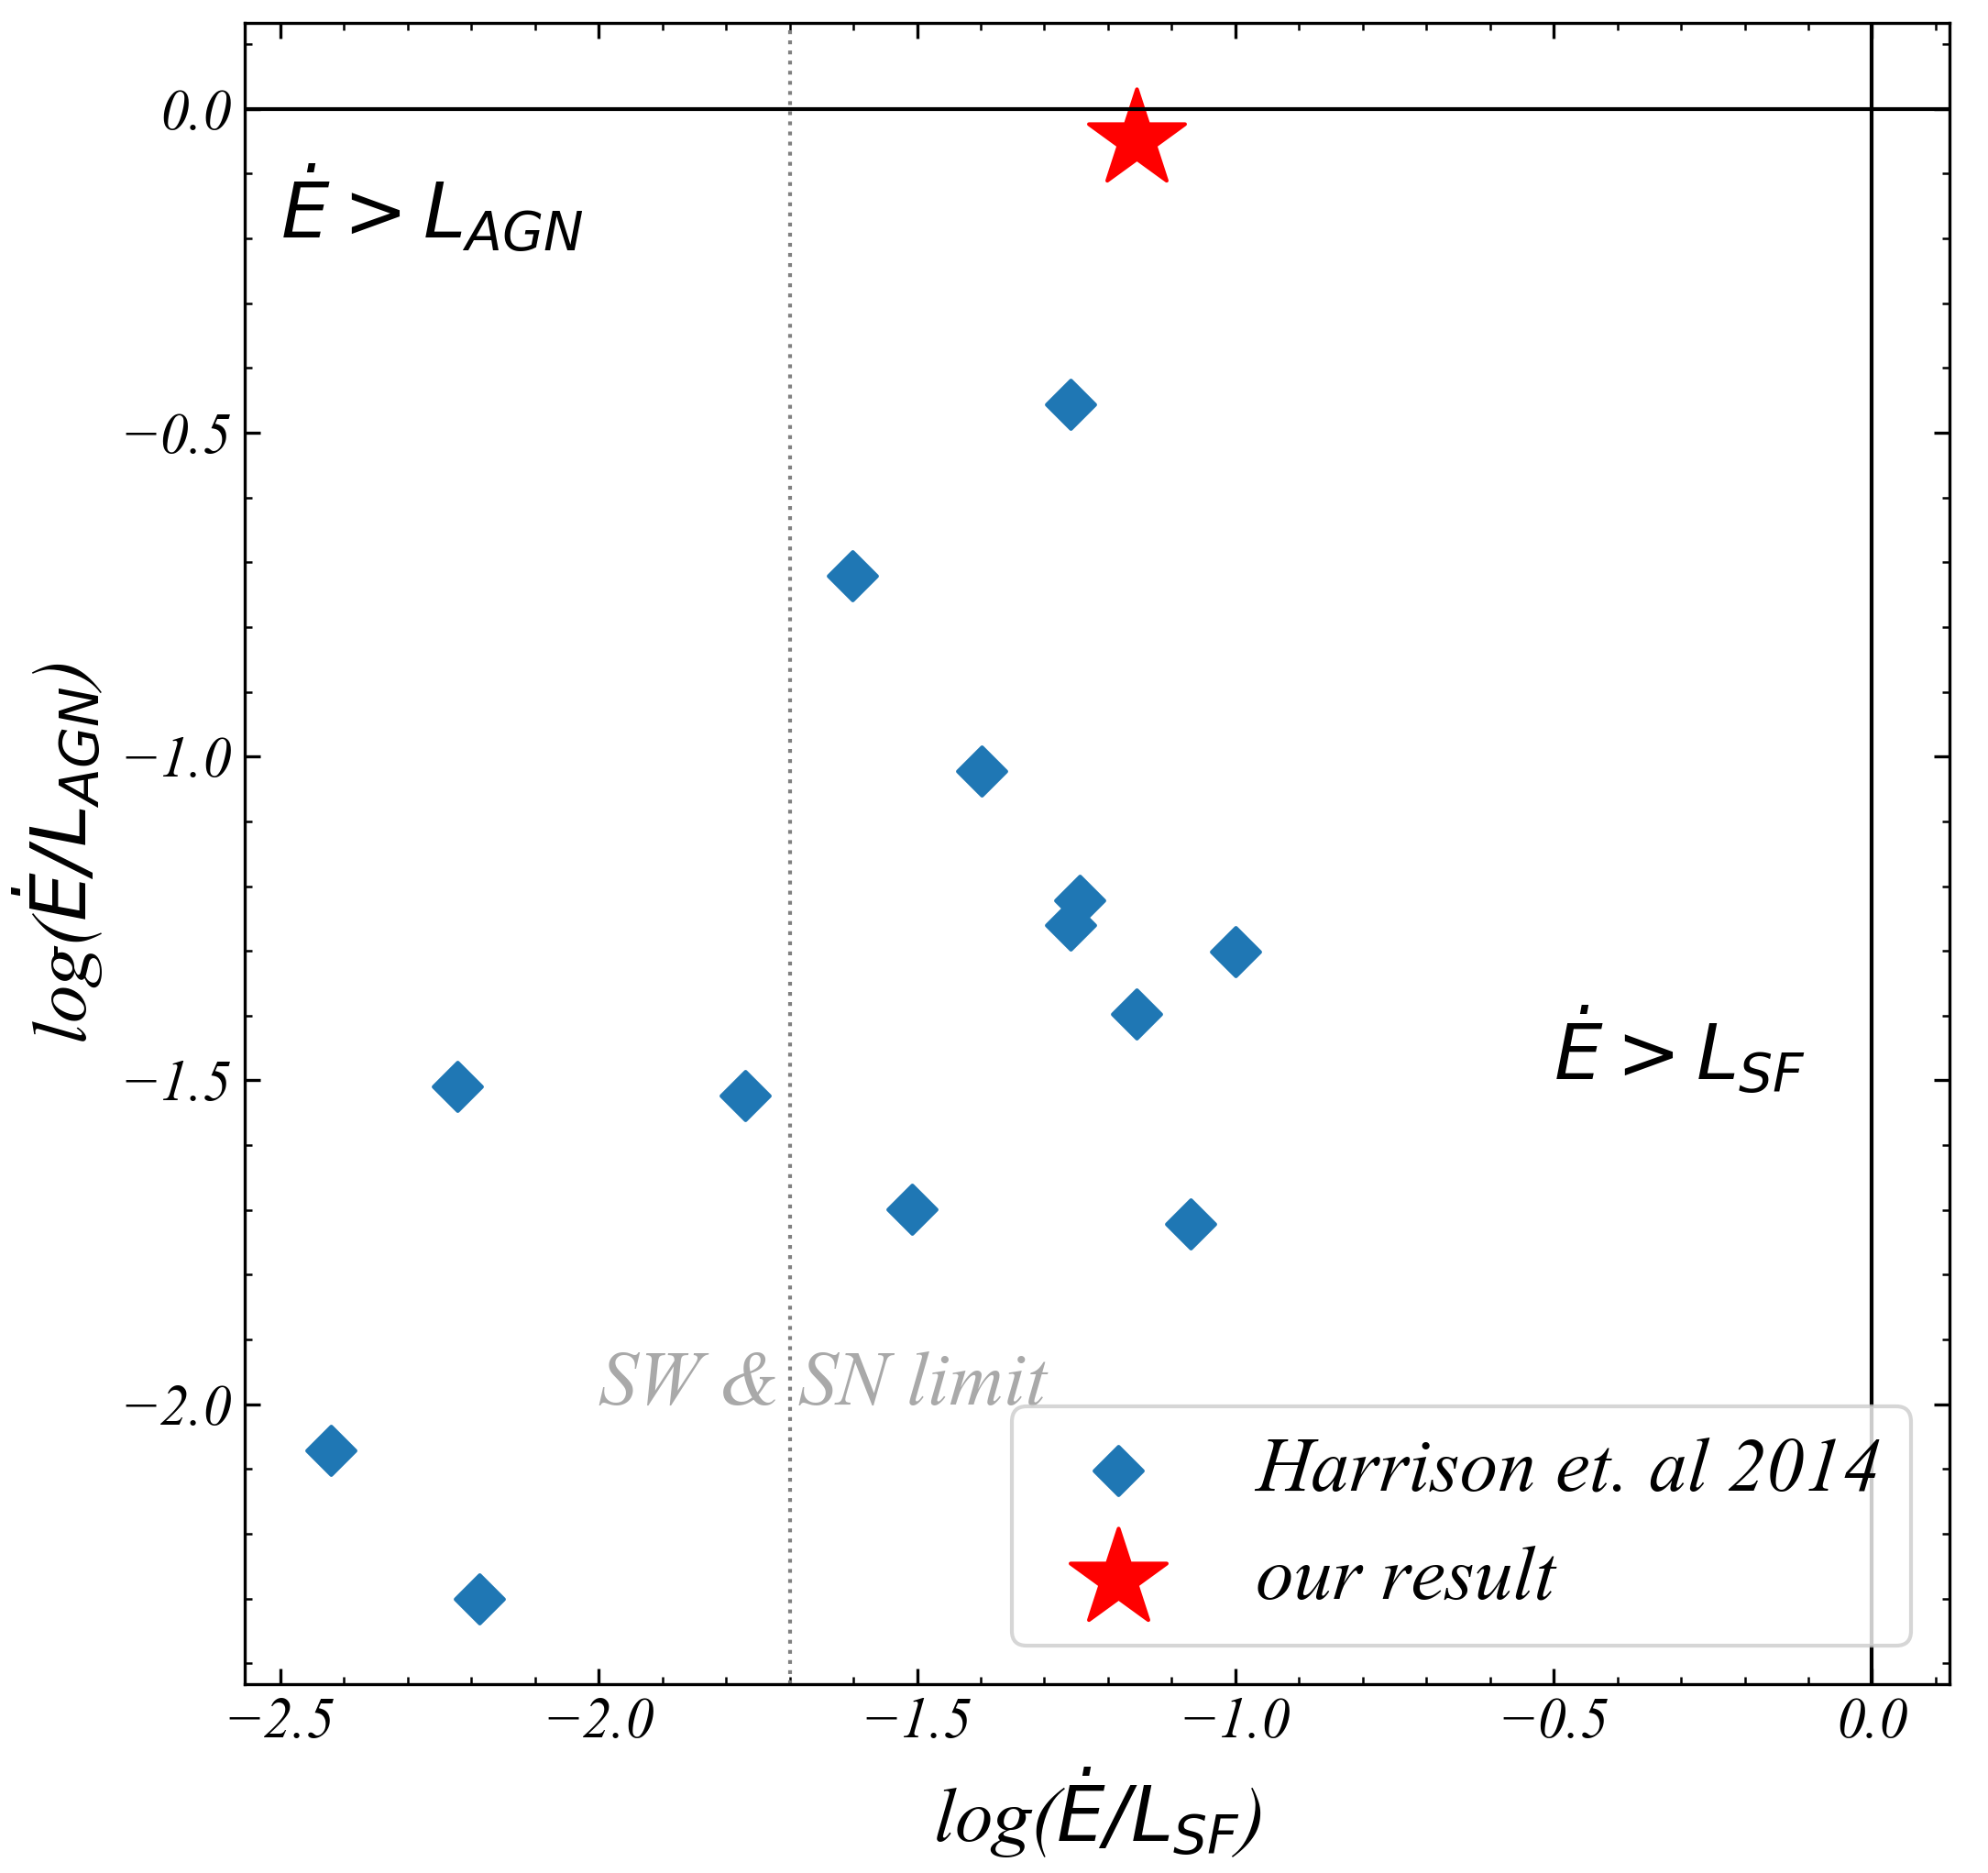
\includegraphics[width=0.5\textwidth]{figs/cp_AGN_vs_cp_SF}}
		\subfloat{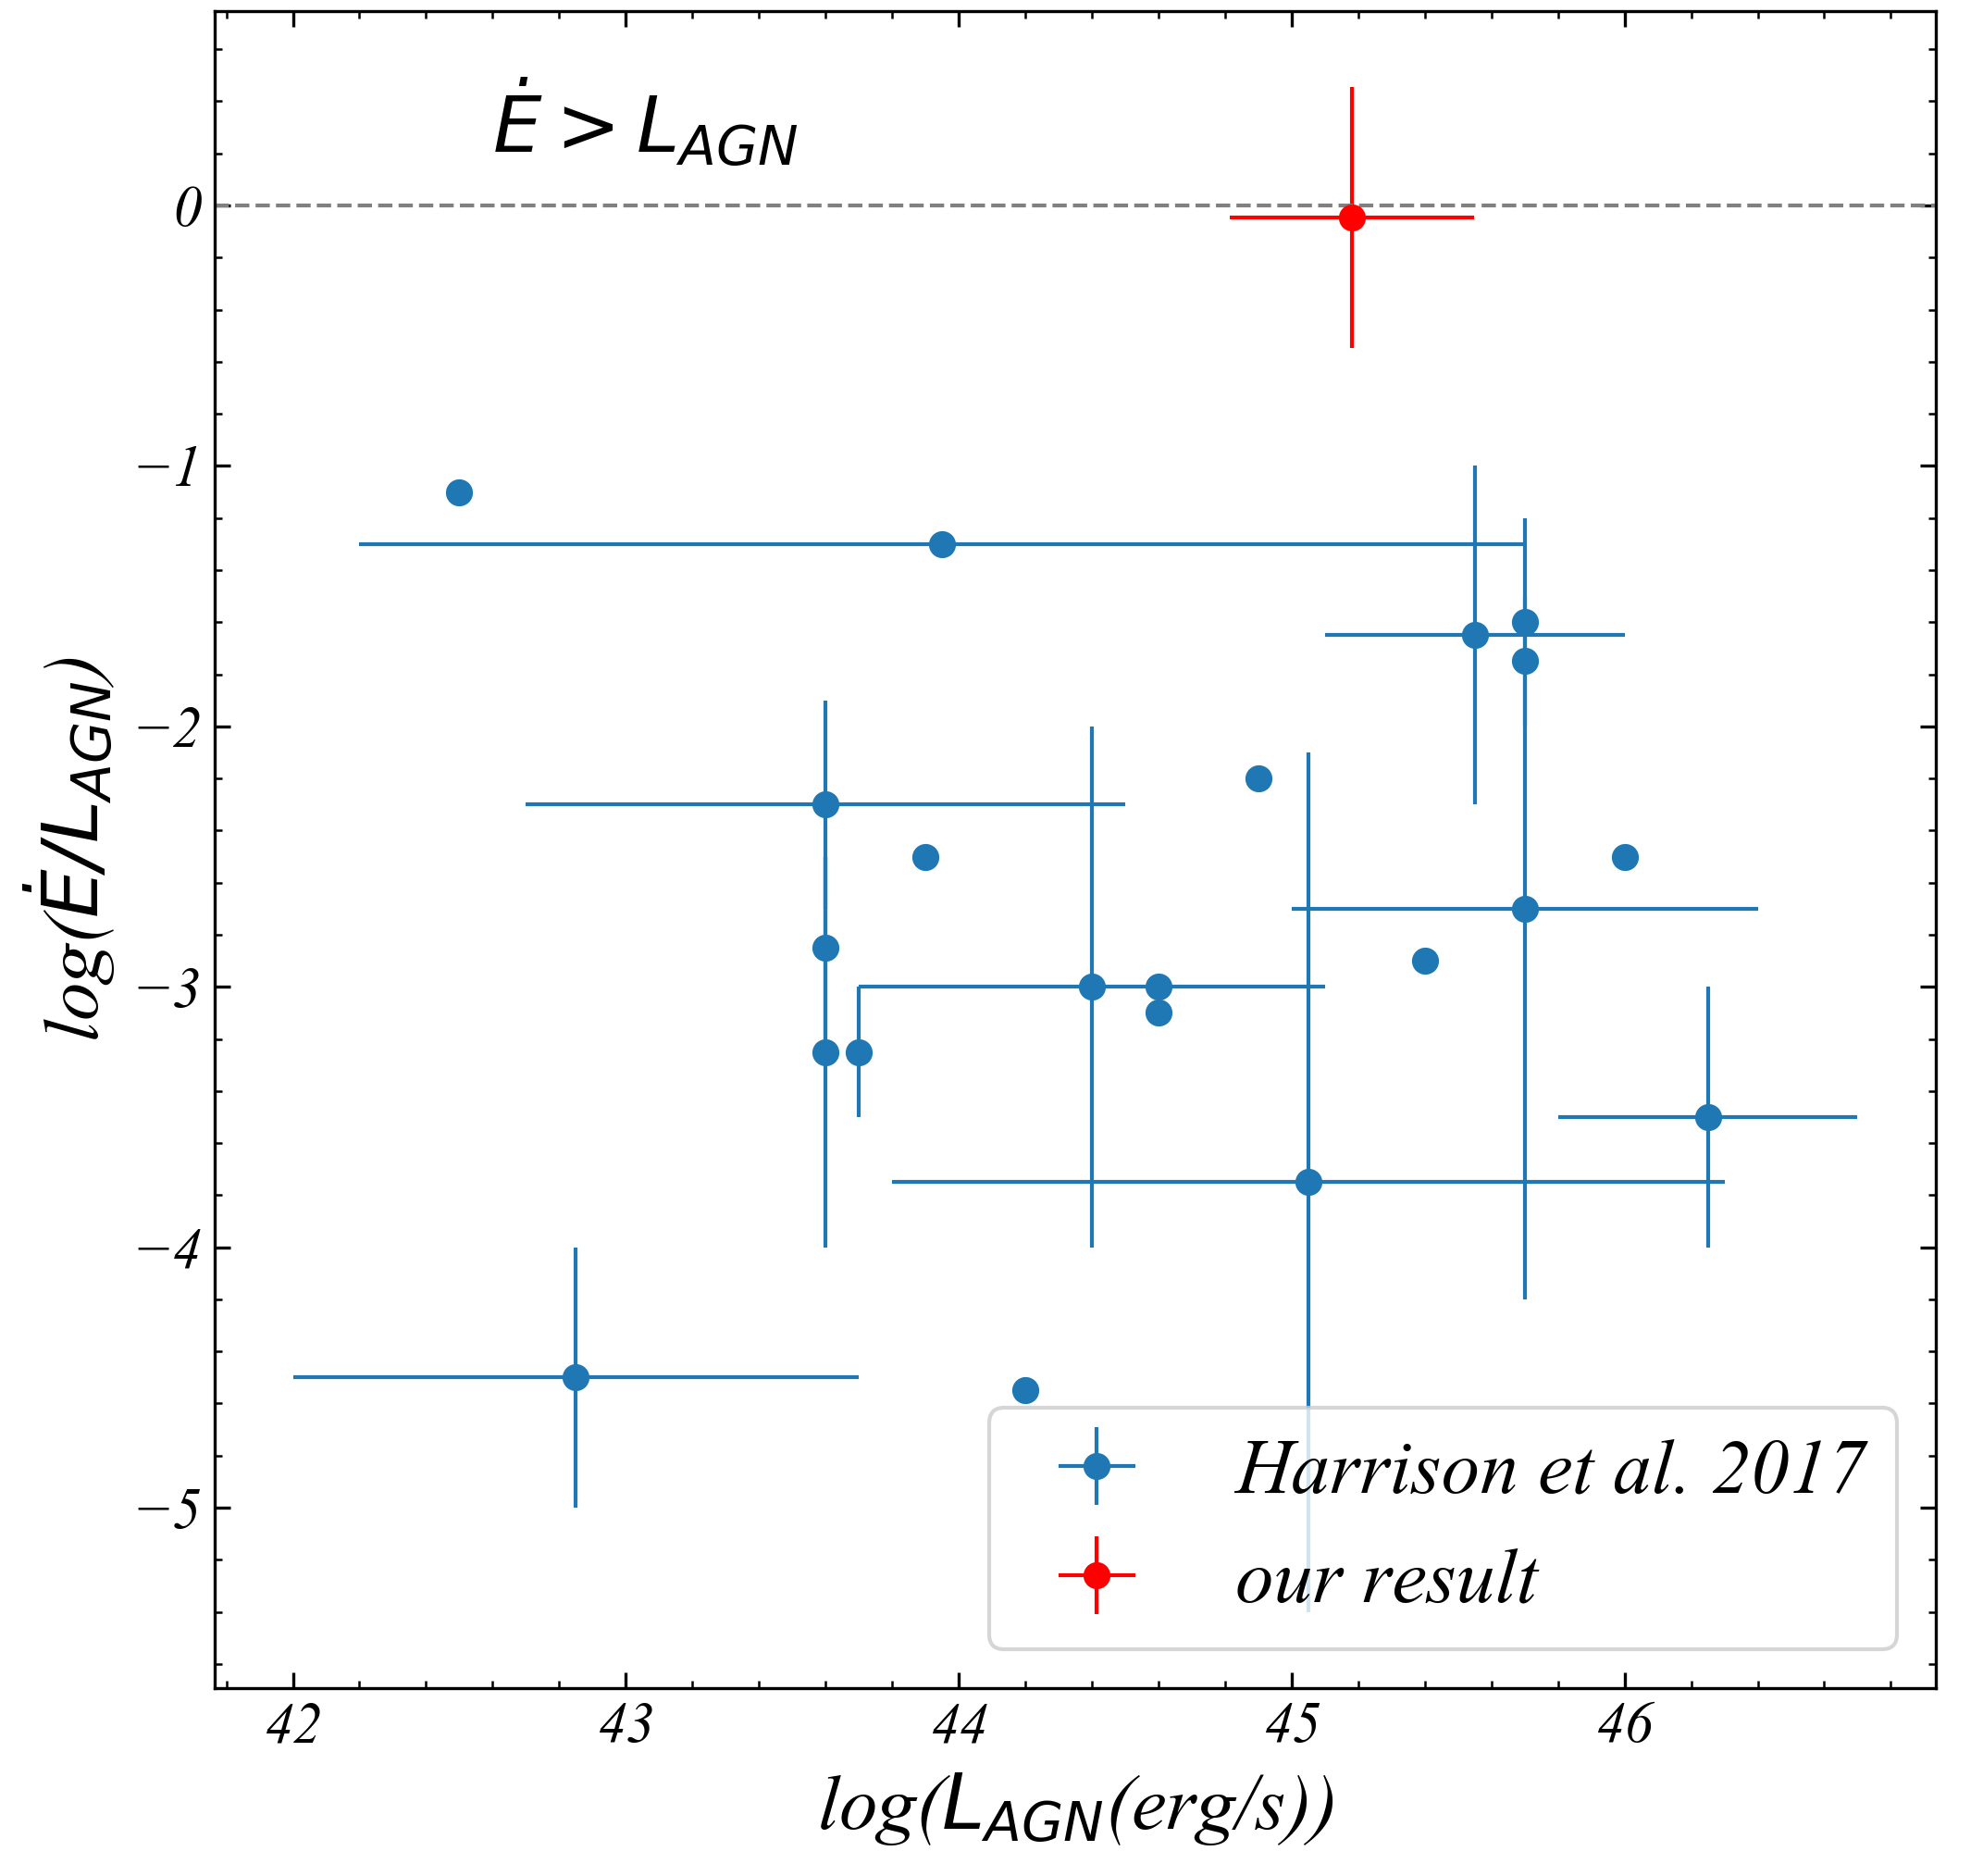
\includegraphics[width=0.5\textwidth]{figs/cp_AGN_vs_L_AGN}}
		\label{coupeffic}
		\caption{Left: the ratio of our estimated outflow kinetic energy rates($E_{out}$) to the AGN luminosity and to the star formation luminosity for our source(red) and sources from \citet{harrison2014kiloparsec}. The dashed vertical line is the estimated maximum mechanical input expected from supernovae and stellar winds. The two solid lines shows the coupling efficiency of 1. Right: Observationally determined kinetic coupling efficiencies in \citet{harrison2018agn} and our result. The vertical lines show the range of values quoted or, in the case of an error bar, the quoted error on the average value. The horizontal lines show the range of bolometric luminosity for each sample. The dotted line shows coupling efficiency of 1. }
	\end{figure*}
	
	In this section we will investigate which of these processes could be responsible for driving the extreme outflows observed. The dominant processes that drive such large scale outflow in protocluster and the efficiency to which they are able to couple the gas are currently sources of uncertainty in galaxy formation models. Several possible mechanisms have been suggested to drive galaxy-wide outflows, for example: the stellar wind and supernovae; radiation pressure from the extremely luminous AGN or star formation; the interaction of radio jets with a clumpy and multiphase interstellar medium; AGN wind initially launched from the accretion disc. Following \citet{harrison2014kiloparsec}, we calculate the coupling efficiency which is a popular method to investigate the likely drivers of large-scale outflow. We compare the ratio of our outflow kinetic energy rate ($\rm \dot{E_{out}}$) with (1) the AGN bolometric luminosity converted from AGN IR luminosity; (2) the star formation luminosity \citep{arrigoni2018overdensity}. We also calculate the momentum-loading factor for both star-forming-driven case and AGN-driven case. Using these results we now explore the possible driving mechanisms to power this outflow. 
	 
	 Fig.\ref{coupeffic} shows coupling efficiency for both star-forming-driven case and AGN-driven case. We compare our result with results in \citet{harrison2014kiloparsec}. One way for star formation to drive large-scale outflow is by stellar winds or supernovae. An estimation of the coupling efficiency for this case is carried by \citet{kennicutt1998star}, he found that the maximum coupling efficiency is $\rm \dot{E_{out}}/L_{IR,SF} \approx 0.02$, we indicate this upper limit with gray dot line in Fig.\ref{coupeffic}. Based on this result, stellar winds and supernovae are unlikely to be fully responsible to power outflow on physical scale of 100 kpc. By adopting a potential model for a halo with stellar mass $\rm M_{*}=3 \times 10^{11} M_{\odot}$ at $\rm z \approx 2$ we run stellar feedback simulation, it shows the initial outflow velocity should reach 2300 km/s to meet our observation. However, neither of \citet{Heckman2016The} nor \citet{Li_2020} shows stellar feedback can power such larger initial velocity which also indicates stellar formation is not a good interpretation for our case. On the other hand, the coupling efficiency for AGN-driven case is too large which is close to 1. In the right panel of Fig.\ref{coupeffic} it shows that if the outflow is driven by AGN, it has already exceed other results with similar AGN luminosity. 
	 
	 Besides, if we instead consider a momentum-driven wind with momentum deposition from the radiation pressure of stars or AGN, the momentum loading factors are $\rm f_{p,SF}=1.7$ and $\rm f_{p,AGN}=3.2$ for the two mechanisms. Nevertheless \citet{zubovas2018agn} suggests that a typical momentum loading factor for star-formation-driven case is $\rm f_{p,SF}< 1.4$ which is lower than our estimation, this comparison also rules out the star-formation case. In the same way, we also find that $\rm f_{p,AGN}$ is larger than the typical value. 
	 
	 Moreover, \citet{shankar2006new} mentions the two sources of feedback have different effects over different mass ranges, in particular, stellar feedback regulates the processes in low-mass galaxies while large galaxies are mainly regulated by AGN feedback. The transition mass for this two feedback mechanisms is $\rm M_{tr} \approx 2 \times 10^{10} \mathrm{M}_{\odot} $. By fitting the SED of source-B, \citet{arrigoni2018qso} estimates its stellar mass of source-B to be $\rm \log \left(M_{\mathrm{star}} / M_{\odot}\right)=11.4_{-0.2}^{+0.3}$. Comparing with $\rm M_{tr}$, it also confirms star-forming driven feedback is not the possible mechanism to power this outflow.
	 
	 However, \citet{zubovas2018agn} also suggests there are mechanisms to reach high coupling efficiency and momentum loading factor. One possibility is hyper-Eddington Super Massive Black Hole (SMBH) growth during Compton-thick (heavily obscured) phase. In this case, SMBH would accrete material with extremely large rate and may lead to ultra fast outflows (UFO).  \citet{tombesi2013unification} shows the initial velocity is able to reach to $\rm 0.1c$ and will have a strong coupling with the interstellar medium (ISM). Fig.6 of \citet{tombesi2013unification} shows the coupling efficiencies approximate 1 for some cases, but he also explains that this extremely fast and powerful outflow would occur only very close to SMBH $\rm R \approx 1000r_{s}$ (where $\rm r_{s}$ is the schwarzschild radius.).  He indicates that the large coupling efficiency is probably due to large environment column density $\rm \approx 10^{24} \ cm^{-2}$ and highly ionized state which is similar to the large-scale environmental conditions of MAMMOTH-1. \citet{cai2017discovery} suggests that the hydrogen column density is in the range $\rm 10^{20} \ cm^{-2}$, with the presence of highly-coupling outflow we indicate here that the column density in CGM maybe $\rm 10^{3} cm^{-2}$ larger than this value. 
	 
	 In summary, based on above analyses we find MAMMOTH-1 outflow is likely to be powered by AGN wind during the hyper-Eddington accretion of SMBH instead of star-forming processes. Although there is large uncertainty in the estimation of coupling efficiency, the very-large-scale-effecting feedback is never observed before. If it is true, our result should be the first observation of AGN-mode feedback on 100 kpc. It puts a very strong constrain on galaxies feedback processes and even further affects our understanding of galaxy evolution.

\end{document}